\documentclass[conference]{IEEEtran}
\IEEEoverridecommandlockouts
% The preceding line is only needed to identify funding in the first footnote. If that is unneeded, please comment it out.
\usepackage{cite}
\usepackage{amsmath,amssymb,amsfonts}
\usepackage{algorithmic}
\usepackage{graphicx}
\usepackage{textcomp}
\usepackage{xcolor}
\usepackage{color}
\usepackage{listings}
\usepackage{xparse}
\usepackage[spaces,hyphens]{url}
\usepackage{hyperref}

\def\BibTeX{{\rm B\kern-.05em{\sc i\kern-.025em b}\kern-.08em
    T\kern-.1667em\lower.7ex\hbox{E}\kern-.125emX}}
    
\NewDocumentCommand{\codeword}{v}{%
\texttt{\textcolor{blue}{#1}}%
}

\NewDocumentCommand{\tool}{v}{%
\texttt{\textcolor{gray}{#1}}%
}

% path gambar
\graphicspath{{../Gambar/}}

\lstset{language=Bash,keywordstyle={\bfseries \color{blue}}}

\hypersetup{
    colorlinks=true,
    linkcolor=blue,
    filecolor=magenta,      
    urlcolor=cyan,
    pdftitle={Overleaf Example},
    pdfpagemode=FullScreen,
    }
    
\definecolor{dkgreen}{rgb}{0,0.6,0}
\definecolor{gray}{rgb}{0.5,0.5,0.5}
\definecolor{mauve}{rgb}{0.58,0,0.82}

\lstset{frame=tb,
  language=Bash,
  aboveskip=3mm,
  belowskip=3mm,
  showstringspaces=false,
  columns=flexible,
  basicstyle={\small\ttfamily},
  numbers=none,
  numberstyle=\tiny\color{gray},
  keywordstyle=\color{blue},
  commentstyle=\color{dkgreen},
  stringstyle=\color{mauve},
  breaklines=true,
  breakatwhitespace=true,
  tabsize=3
}

\begin{document}

\title{Implementasi WiFi Scanner Dengan NodeMCU dan Integrasi Bot Telegram}

\author{\IEEEauthorblockN{Ricky}
	\IEEEauthorblockA{\textit{Teknik Komputer, Fakultas Teknologi Informasi} \\
		\textit{Institut Teknologi Batam}\\
		Batam, Indonesia \\
		1922022@student.iteba.ac.id}
	\and
	\IEEEauthorblockN{Muhamad Arie}
	\IEEEauthorblockA{\textit{Teknik Komputer, Fakultas Teknologi Informasi} \\
		\textit{Institut Teknologi Batam}\\
		Batam, Indonesia \\
		1922021@student.iteba.ac.id}
}
\maketitle

\begin{abstract}
	Wifi Scanner adalah sebuah proyek yang bertujuan untuk mengukur kekuatan sinyal wifi di area terdekat dan melaporkannya ke Telegram bot chanel.
\end{abstract}

\begin{IEEEkeywords}
	Simulation, Networking, Detection, Scanner
\end{IEEEkeywords}

\section{Pengenalan}
Pada saat ini teknologi nirkabel sudah sangat umum, salah satunya seperti Wireless Fidelity atau WiFi. Diperkenalkan pada tahun 1998 yang juga distandarisasi oleh Institute of Electrical and Electronics Engineers (IEEE) 802.11. Teknologi ini memungkinkan untuk mengirim data antar client dalam satu cakupan jaringan lokal. Pada dasarnya konsep WiFi menggunakan antena pemancar (transmitter) dan penerima (receiver). Pemancar disini akan memancarkan gelombang radio Pada kesempatan ini kami bertujuan untuk mengukur kekuatan dari sinyal dan melakukan sedikit uji coba dengan menambahkan beberapa hambatan antara pemancar dan penerima sinyal.

\section{Tools}\label{teori-tool}

\subsection{NodeMCU ESP 8266}
NodeMCU adalah firmware dan papan pengembangan berbasis Lua open-source yang ditargetkan khusus untuk Aplikasi berbasis IoT. Ini termasuk firmware yang berjalan pada SoC Wi-Fi ESP8266 dari Sistem Espressif, dan perangkat keras yang didasarkan pada modul ESP-12.

\begin{figure}[h]
  \centering
  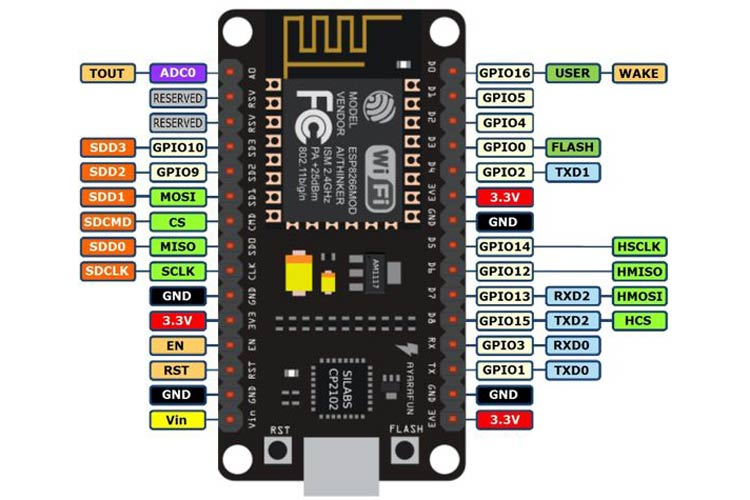
\includegraphics[width=0.38\textwidth]{esp8266.jpg}
  \caption{nodeMCU Schema}
\end{figure}

\subsection{Telegram and Bot Father}
Telegram adalah layanan pesan instan berbasis cloud, lintas platform, freemium. Layanan ini juga menyediakan panggilan video terenkripsi ujung ke ujung, VoIP, berbagi file, dan beberapa fitur lainnya. Diluncurkan untuk iOS pada 14 Agustus 2013 dan Android pada 20 Oktober 2013. Server Telegram didistribusikan di seluruh dunia dengan lima pusat data di berbagai wilayah, sedangkan pusat operasional berbasis di Dubai, Uni Emirat Arab. Berbagai aplikasi klien tersedia untuk platform desktop dan seluler termasuk aplikasi resmi untuk Android, iOS, Windows, macOS, dan Linux. Ada juga dua aplikasi kembar web Telegram resmi, WebK dan WebZ, dan banyak klien tidak resmi yang menggunakan protokol Telegram. Semua komponen resmi Telegram adalah open source, kecuali server yang bersifat closed-source dan proprietary. Telegram menyediakan obrolan terenkripsi ujung-ke-ujung opsional.

\begin{figure}[h]
  \centering
  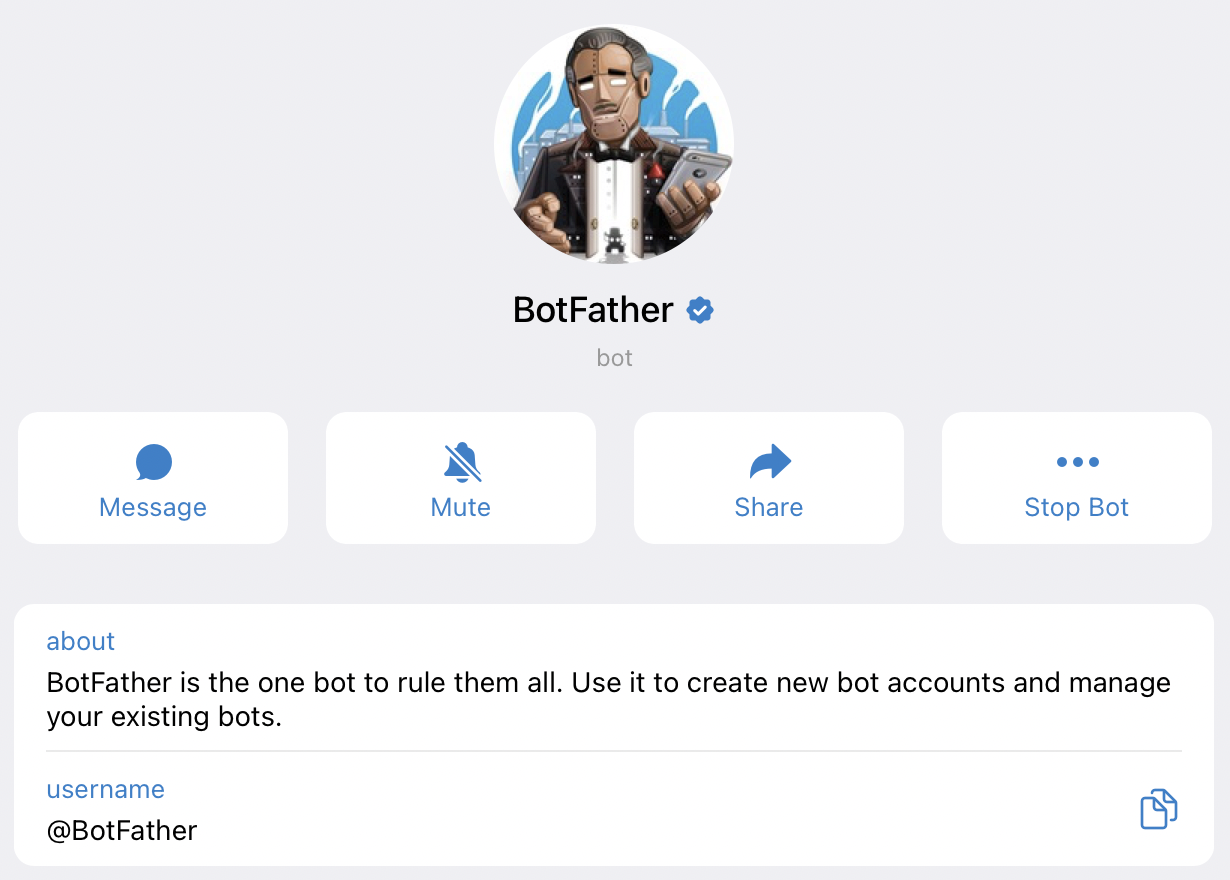
\includegraphics[width=0.38\textwidth]{botfather.png}
  \caption{Telegram Bot Father}
\end{figure}

\subsection{Aplikasi Arduino}
Aplikasi Arduino digunakan untuk menulis firmware untuk NodeMCU, kita dapat memprogram untuk terhubung ke jaringan local agar NodeMCU nantinya dapat mengirimkan hasil pemindaian ke webserver gateway relay yang akan meneruskan ke bot Telegram.

\subsection{Laravel}
Laravel adalah kerangka kerja aplikasi web berbasis PHP yang sumber terbuka, menggunakan konsep Model-View-Controller (MVC). Laravel berada dibawah lisensi MIT, dengan menggunakan GitHub sebagai tempat berbagi kode (Code Base). Kami menggunakan Laravel sebagai teknologi utama dalam pemrograman web gateway penerima hasil pemindaian sinyal WiFi yang nantinya akan diteruskan ke bot Telegram.

\section{Pengerjaan}\label{pengerjaan}
Pengerjaan dimulai dari menginstall web framework laravel lalu mencari source code program untuk nodemcu firmware dan flash firware menggunakan aplikasi Arduino ke nodemcu. Selanjutnya menghidupkan nodemcu agar terhubung ke lokal WiFi agar dapat internet akses, dan juga kita perlu menjalankan lokal webserver untuk menerima data dari arduino. Adapun beberapa kondisi yang kami uji cobakan adalah sebagai berikut:

\subsection{Uji coba case 1}

\begin{itemize}
  \item Scanner berada di dalam ruangan
  \item Target WiFi area berada diluar ruangan
  \item Terhalang tembok setebal 7cm 
  \item Memiliki 1 pintu dengan 2 jendela kaca standard
  \item Lebar ruangan 2,12m x 2,88m
\end{itemize}

\begin{figure}[h]
  \centering
  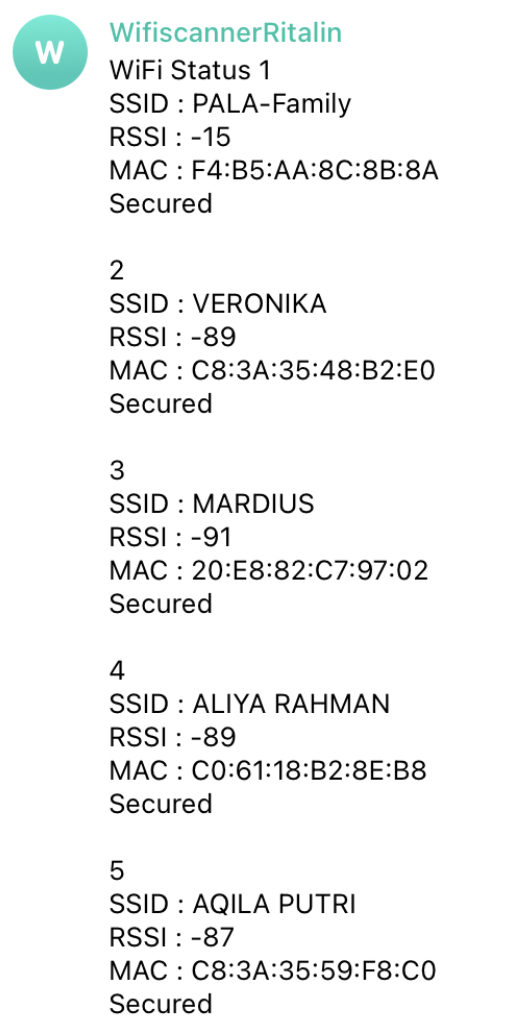
\includegraphics[width=0.30\textwidth]{scanning-result.png}
  \caption{Scanning Result 1, tidak ada target yang berada dalam satu ruangan}
\end{figure}


\subsection{Uji coba case 2}

\begin{itemize}
  \item Scanner berada di dalam ruangan
  \item Target WiFi area berada diluar ruangan dan dalam ruangan
  \item Terhalang tembok setebal 7cm 
  \item Memiliki 1 pintu dengan 2 jendela kaca standard
  \item Lebar ruangan 2,12m x 2,88m
  \item SSID: PALA-Family merupakan Router ZTE-F609
  \item SSID: ARES merupakan Hotspot Nirkabel iPhone 11
\end{itemize}

\begin{figure}[h]
  \centering
  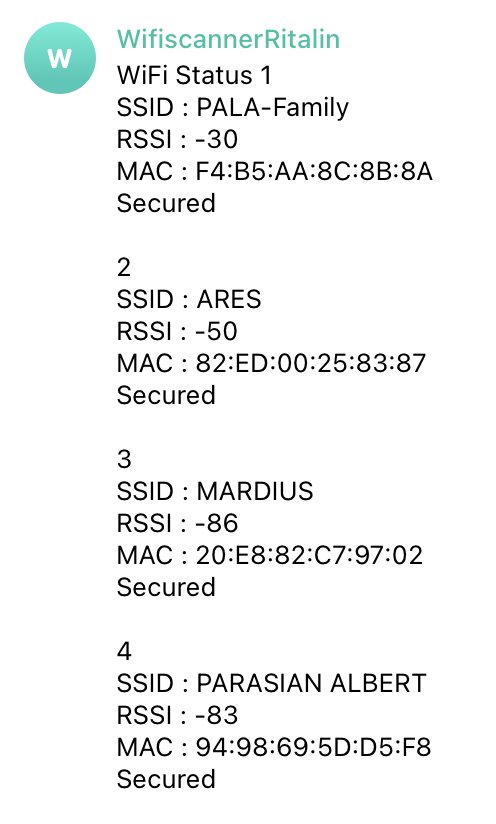
\includegraphics[width=0.30\textwidth]{scanning-result2.png}
  \caption{Scanning Result 2, SSID ARES adalah target yang berada dalam satu ruangan}
\end{figure}

\textit{Figure 4}, Seperti yang dapat dilihat, SSID: PALA-Family memiliki sinyal yang lebih kuat dikarenakan Transmitter WiFi menggunakan antena yang lebih panjang.

\section{Kesimpulan}

Gelombang WiFi adalah jenis radio frekuensi yang merambat melalui udara, jika udara terhambat oleh objek. Dalam kasus pengetesan ini objek berupa tembok dan kaca jendela, maka kekuatan pemancaran WiFi juga dapat melemah begitupun sebaliknya. Faktor lain yang dapat mempengaruhi kekuatan sinyal yaitu pemancar(transmitter) penerima(receiver) sinyal itu sendiri, semakin bagus devicenya semakin kuat pula sinyal WiFi tersebut.
\end{document}